\documentclass[11pt]{article}

\usepackage{polski}
\usepackage{geometry}
	\geometry{margin = 2.5cm}
\usepackage{indentfirst}
\usepackage{xcolor}
\usepackage{bold-extra}
\usepackage[T1]{fontenc}
\usepackage[utf8]{inputenc}
\usepackage{palatino}
\usepackage{graphicx}
\usepackage[unicode]{hyperref}
\usepackage{fancyhdr}
\usepackage{multirow}
\usepackage{listings}
\usepackage[shortlabels]{enumitem}
	\setlist[itemize]{--, itemsep = 0cm}
\usepackage{amsmath}
\usepackage{subfig}
\usepackage[title]{appendix}

\linespread{1.25}

\definecolor{codegray}{rgb}{0.5, 0.5, 0.5}
\definecolor{codepurple}{rgb}{0.58, 0, 0.82}
\definecolor{backcolour}{rgb}{0.95, 0.95, 0.92}

\lstdefinestyle{mystyle}{%
	backgroundcolor = \color{backcolour},
%	basicstyle = \ttfamily \small,
 	basicstyle = \ttfamily \footnotesize,
	commentstyle = \color{green!50!black},
	numberstyle = \tiny \color{codegray},
	stringstyle = \color{codepurple},
	keywordstyle = \color{blue!85!black},
	breakatwhitespace = false,
	breaklines = true,
	captionpos = b,
	keepspaces = true,
	showspaces = false,
	showstringspaces = false,
	showtabs = false,
	tabsize = 4,
	numbers = left,
	numberstyle = \tiny \color{black},
	morecomment = [l]{//},
	frame = single
}

\lstset{%
	style = mystyle,%
	language = C,
	morekeywords = {byte},
	literate = %
		{ą}{{\k{a}}}1
		{Ą}{{\k{A}}}1
		{ć}{{\'c}}1
		{Ć}{{\'{C}}}1
		{ę}{{\k{e}}}1
		{Ę}{{\k{E}}}1
		{ł}{{\l{}}}1
		{Ł}{{\L{}}}1
		{ń}{{\'n}}1
		{Ń}{{\'N}}1
		{ó}{{\'o}}1
		{Ó}{{\'O}}1
		{ś}{{\'s}}1
		{Ś}{{\'S}}1
		{ż}{{\.z}}1
		{Ż}{{\.Z}}1
		{ź}{{\'z}}1
		{Ź}{{\'Z}}1
}

\pagestyle{fancy}
\fancyhf{}
\lhead{SWiSCR -- Line follower}
\rhead{Skibiński, Kaźmieruk}
\cfoot{\thepage}

\graphicspath{{./img/} {./img/foto/}}



%%%
%%%		DOKUMENT
%%%

\begin{document}



%%%
%%%		TITLEPAGE
%%%

\begin{titlepage}
{\LARGE
\begin{center}
	\begin{figure}[h!]
		\centering
		\includegraphics[width = 0.2\linewidth]{C:/good_folder/nauka/inne/polsl_logo_v2}
	\end{figure}
	
	\vspace{0.25cm}
	
	\textbf{\textsc{Politechnika Śląska}}
	
	\textbf{\textsc{Wydział Automatyki, Elektroniki i Informatyki}}
	
	\vspace{1.5cm}
	
	Projekt z przedmiotu Systemy Wbudowane i Systemy\linebreak Czasu Rzeczywistego
	
	\vspace{1.5cm}
	
	\textbf{Line follower}
\end{center}
}

\vfill

{\Large
\noindent \textbf{Autorzy}:\\
\hspace*{0.5cm} inż. Maksymilian Skibiński\\
\hspace*{0.5cm} inż. Paweł Kaźmieruk\\
rok 2020/2021, sem. letni, gr. Rob, sekcja nr 1

\vspace{0.5cm}

\noindent \textbf{Kierujący pracą}:\\
\hspace*{0.5cm} dr inż. Krzysztof Jaskot

\vspace{0.5cm}
}

\begin{center}
Gliwice, lipiec 2021
\end{center}
\end{titlepage}




%%%
%%%		CONTENT
%%%

\setcounter{page}{2}

\tableofcontents

\newpage

\section{Wstęp}

Celem projektu była budowa i zaprogramowanie mobilnego robota poruszającego się wzdłuż linii, tzw. Line followera.
W dużym skrócie, taki pojazd jest wyposażony w odpowiednie czujniki, które informują mikrokontroler o jego położeniu w stosunku do linii, a ten korzystając z tej wiedzy generuje odpowiednie sygnały modyfikujące prędkości jego kół.
W ten sposób robot potrafi podążać za swoją trasą.

Sposobów na realizację tego zadania jest wiele i zależy to już w głównej mierze od autorów projektu. Treścią tego raportu jest omówienie jednego z takich pomysłów, który został zrealizowany przez autorów.

Jako etapy realizacji projektu można wymienić:
\begin{itemize}
\item projekt części elektronicznej projektu: wybór czujników, mikrokontrolera, wybór silników oraz kół, okablowanie,
\item projekt podwozia wraz z instalacją całego osprzętu,
\item propozycja systemu sterowania i jego implementacja w systemie wbudowanym oraz systemie czasu rzeczywistego,
\item wnioski końcowe, pomysły na przyszłość.
\end{itemize}
 


\newpage

\section{Harmonogram}

Zajęcia odbywały się w trzecim bloku zajęć w semestrze. Składało się na nie 5 cotygodniowych wirtualnych spotkań, podczas których pokazywane były postępy w pracy. Projekt był wykonywany pomiędzy tymi spotkaniami.

\subsubsection*{Tydzień 1}

Na pierwsze spotkanie przygotowany został robot, który potrafił się poruszać, ale wykonywał tylko zaprogramowane ruchy. Na tym etapie nie posiadał żadnej autonomii i nie potrafił jeździć wzdłuż trasy.

\subsubsection*{Tydzień 2}

Z powodów godzin dziekańskich te zajęcia się nie odbyły.

\subsubsection*{Tydzień 3}

Tym razem, robot potrafił już jeździć wzdłuż linii. Zainstalowane zostały dwa analogowe sensory na przodzie pojazdu informujące o jego położeniu względem linii oraz zaimplementowane zostało prawo sterowania, które korzystając z różnicy tych wskazań generowało odpowiedni (proporcjonalny do niej) sygnał sterujący.

Robot poruszał się płynnie i z zadowalającą prędkością wzdłuż trasy, potrafił pokonywać mniej lub bardziej ostre zakręty oraz nie było dla niego problematyczne skrzyżowanie na środku trasy, ale nie potrafił wykonać skrętu o 90 stopni. Dwa czujniki okazały się do tego niewystarczające (choć być może zdolniejsi nawet z nich umieją zrealizować to zadanie).

Na tym etapie powstał też całkiem ciekawy pomysł zainspirowany naturą -- a dokładniej rybami głębinowymi -- kupna jeszcze jednego czujnika analogowego, który celowo miał wystawać przed pojazd i informować o przyszłych zmianach na trasie. Ostatecznie jednak, ze względu na inne bardziej istotne problemy, ten pomysł nie został zrealizowany.\\

Materiały prezentujące działanie robota na tym etapie:
\begin{itemize}
\item \href{https://youtu.be/KM7RJapF71Y}{https://youtu.be/KM7RJapF71Y}
\item \href{https://youtu.be/R2dgWDf-asg}{https://youtu.be/R2dgWDf-asg}
\end{itemize}

\subsubsection*{Tydzień 4}

Dołożone zostały dwa kolejne czujniki, tym razem cyfrowe, na przód pojazdu, za pomocą których robot był w stanie wykonywać skręty o 90 stopni. Pewnej zmianie musiało ulec prawo sterowania (które dokładniej zostanie omówione później), dodany został człon D do regulacji (czyli na tym etapie działało równanie PD), ale co najważniejsze dodanie kolejnych czujników nie wpłynęło negatywnie na płynny ruch robota po trasie, a tylko pomogło przy ostrych skrętach.

Na tym etapie, pojazd już spełniał swój cel -- potrafił podążać za linią.\\

Materiały prezentujące działanie robota na tym etapie:
\begin{itemize}
\item \href{https://youtu.be/qdXwQmjnL98}{https://youtu.be/qdXwQmjnL98}
\item \href{https://youtu.be/QG8gyqzkxBA}{https://youtu.be/QG8gyqzkxBA}
\end{itemize}

\subsubsection*{Tydzień 5}

Ostatni tydzień poświęcony został głównie na zapoznanie się z systemem czasu rzeczywistego\linebreak FreeRTOS oraz na implementację układu sterowania w tym systemie. Jak ostatnie zajęcia pokazały -- cel został zrealizowany.

Pewnym zmianom uległy także zmiany nastaw regulatora PD oraz działanie trybu nawracania -- robot nie robi teraz obrotu o 90 stopni w miejscu, tylko skręca oraz wraca do tyłu, by nadrobić to, że drobno wyjechał poza trasę.\\

Materiały prezentujące działanie robota pod koniec zajęć projektowych:
\begin{itemize}
\item \href{https://youtu.be/4WTrk285v4s}{https://youtu.be/4WTrk285v4s}
\item \href{https://youtu.be/nwpjGGdDjxc}{https://youtu.be/nwpjGGdDjxc}
\end{itemize}

\newpage

\section{Elementy}

\subsection{Kosztorys}

By projekt mógł zostać wykonany, konieczne było kupno wielu części.
Te zostały spisane w podanej poniżej tabeli nr \ref{table:kosztorys}.

\begin{table}[h!]
	\centering
	\begin{tabular}{|c||c|}
		\hline
		FORBOT -- zestaw do budowy robota & \textbf{270 zł} \\
		\hline
		Arduino Uno Rev3 & \textbf{95 zł} \\
		\hline
		Zestaw przewodów połączeniowych -- żeńsko-żeńskie & \textbf{6 zł} \\
		\hline
		Czujnik odległości, odbiciowy 3,3V/5V - Iduino ST1140 & 2 x \textbf{7,70 zł} \\
		\hline
		Bateria AA (R6 LR06) alkaliczna Energizer Alkaine Power - 4szt. & 2 x \textbf{8,50 zł} \\
		\hline\hline
		\multicolumn{1}{|r||}{\textbf{Suma}\phantom{a}} & \textbf{403,40 zł}\\
		\hline
	\end{tabular}
	\caption{Kosztorys \label{table:kosztorys}}
\end{table}

Robot był budowany według kursu dostępnego w internecie na stronie Forbota:
\begin{quote}
\href{https://forbot.pl/blog/kurs-budowy-robotow-arduino-wstep-spis-tresci-id18935}
{https://forbot.pl/blog/kurs-budowy-robotow-arduino-wstep-spis-tresci-id18935}
\end{quote}

Większość z wykorzystanych i kluczowych dla projektu części jest zawarta w zestawie pochodzącym z tego kursu.
Warto także dodać, że w zestawie znajdują się także inne, nieistotne dla pracy elementy, więc teoretycznie koszt 
zestawu dla opisanego w tej pracy robota powinien być mniejszy, ale jako że nie wszystkie z tych części możemy kupić
osobno podany został koszt całego zestawu.

Cała praca była wykonywana przez obu członków sekcji, zatem każdy z nich poniósł własne koszta i budował własny pojazd. W ten sposób łatwiej było wymieniać się pomysłami, uwagami i wspólnie pracować nad projektem.

Obaj członkowie sekcji posiadali już swoje Arduino Uno i wykorzystywali je w przeszłości, ale jako, że jest one niezbędne do działania projektu, zostało ono także wpisane do listy kosztów.

Wszystkie zakupy zostały zrobione w internetowym sklepie \href{https://botland.com.pl/}{Botland}.

\subsection{Opis części}

Na rysunku nr \ref{fig:forbotCzesci} została pokazana część elementów wchodzących w skład zakupionego zestawu (pozycja nr 1 w kosztorysie).

\begin{figure}[htbp!]
	\centering
	\includegraphics[width = 0.75\linewidth]{forbotCzesci}
	\caption{Część elementów wchodzących w skład zestawu \label{fig:forbotCzesci}}
	Źródło: \href
		{https://forbot.pl/blog/kurs-budowy-robotow-arduino-wstep-spis-tresci-id18935#gallery-3}{kurs Forbota}
\end{figure}

\subsubsection*{Podwozie}

% Rozmiary: dłg = 19cm, szerokość = 12cm i 9cm

Drewniane elementy widoczne na rysunku nr \ref{fig:forbotCzesci} wchodzą w skład podwozia. Są to lekkie części wykonane ze sklejki, zawierające dużą liczbę otworów o różnej wielkości, co pozwala na odpowiednie przygotowanie robota do realizacji celu. 4 z mniejszych części na lewej stronie służą do montażu silników, a większy kawałek w dolnym lewym rogu służy do montażu koszyka z bateriami.

% \newpage

Największy element, który stanowi podwozie ma wymiary:
\begin{itemize}
\item długość: 19 cm,
\item szerokość przodu: 12 cm,
\item szerokość tyłu: 9 cm.
\end{itemize}

\subsubsection*{Podwozie -- montaż}

By przymocować części takie jak np. silniki, Arduino do podwozia wykorzystany został zestaw różnych śrubek, podkładek i tulei dystansowych:
\begin{itemize}
\item śrubki 30mm, 20mm i 6mm,
\item tuleje dystansowe 25mm i 10mm,
\item podkładki, podkładki sprężyste i nakrętki.
\end{itemize}

\subsubsection*{Koło swobodne}

W skład pojazdu wchodzą w sumie 3 koła. Jednym z nich jest mniejsze koło, które zamontowane zostało z tyłu pojazdu i jest przez niego ciągnięte -- takie kółko może się obracać w dowolnym kierunku. Koło działa na zasadzie podobnej do tej znanej z wózków sklepowych.

\subsubsection*{Koła i silniki}

Pozostałymi dwoma kołami są większe, gumowe koła, które są napędzane przez silniki. Te które wchodzą w skład zestawu (i które zostały użyte w omawianej pracy) można kupić oddzielnie
\href{https://botland.com.pl/silniki-dc-katowe-z-przekladnia/16472-kolo-silnik-65x26mm-5v-z-przekladnia-481-przewody.html}{tutaj} za 15 zł (koło + silnik). Użyte elementy są produkowane przez OEM.

Parametry koła:
\begin{itemize}
\item średnica opony: 65 mm,
\item szerokość opony: 26 mm.
\end{itemize}

Parametry silnika z przekładnią:
\begin{itemize}
\item napięcie zasilania: 5 V,
\item pobór prądu: ok. 180 mA,
\item przekładnia 48:1,
\item prędkość obrotowa po przekładni: ok. 80 $\frac{\text{obr}}{\text{min}}$.
\end{itemize}

W pracy nie został wykorzystany enkoder.

Użyte elementy zostały pokazane na rysunku nr \ref{fig:silnikKolo} poniżej.

\begin{figure}[h!]
	\centering
	\includegraphics[width = 0.4\linewidth]{silnikKolo}
	\caption{Zestaw silnika z kołem \label{fig:silnikKolo}}
	Źródło: \href{https://botland.com.pl/silniki-dc-katowe-z-przekladnia/16472-kolo-silnik-65x26mm-5v-z-przekladnia-481-przewody.html}{sklep Botland}
\end{figure}

\subsubsection*{Nakładka do Arduino}

W projekcie została użyta nakładka (inaczej \emph{shield}) do Arduino, która przygotowuje je do pracy z elementami wchodzącymi w skład robota. Została ona pokazana na rysunku nr \ref{fig:shield}.

\begin{figure}[htbp!]
	\centering
	\includegraphics[width = 0.5\linewidth]{shield}
	\caption{Nakładka \label{fig:shield}}
	Źródło: \href{https://forbot.pl/blog/kurs-budowy-robotow-sterownik-robota-arduino-czujniki-id19006#gallery-2}{kurs Forbota}
\end{figure}

Jak sama nazwa wskazuje, nakładkę ,,nakłada'' się na Arduino, w ten sposób wszystkie połączenia z czujnikami czy silnikami wykonuje się poprzez piny na shieldzie.

Nakładka zawiera:
\begin{itemize}
\item mostek-h DRV8835,
\item bezpiecznik polimerowy wielokrotnego użycia,
\item włącznik zasilania,
\item kondensatory ceramiczne do filtracji zakłóceń,
\item zworka zasilania silników (w ten sposób można łączyć Arduino z komputerem nie uruchamiając silników),
\item złącza dla czujników analogowych i cyfrowych,
\item złącza zasilania.
\end{itemize}

\subsubsection*{Czujniki}

\newcommand{\figTwo}{0.24}

% Analog: https://forbot.pl/blog/kurs-budowy-robotow-sterownik-robota-arduino-czujniki-id19006#gallery-24
% Analog: https://forbot.pl/blog/kurs-budowy-robotow-swiatlolub-sterowanie-latarka-id19362#gallery-3
% Cyfrowy: https://botland.com.pl/czujniki-odbiciowe/14274-czujnik-odleglosci-odbiciowy-33v5v-iduino-st1140-5903351242400.html

\begin{figure}[htbp!]
	\centering

	\phantom{%
		\includegraphics[width = \figTwo \linewidth]{sensorAnalog}%
	\hfill%
	}
	\subfloat[analogowy]{%
		\includegraphics[width = \figTwo \linewidth]{sensorAnalog}%
	}%
	\hfill%
	\subfloat[cyfrowy]{%
		\includegraphics[width = \figTwo \linewidth]{sensorDigital}%
	}%
	\phantom{%
		\includegraphics[width = \figTwo \linewidth]{sensorDigital}%
	}
	
	\caption{Czujniki \label{fig:sensors}}
	Źródła: \href{https://forbot.pl/blog/kurs-budowy-robotow-swiatlolub-sterowanie-latarka-id19362#gallery-3}{kurs Forbota}, \href{https://botland.com.pl/czujniki-odbiciowe/14274-czujnik-odleglosci-odbiciowy-33v5v-iduino-st1140-5903351242400.html}{sklep Botland}
\end{figure}


Do wykrywania linii wykorzystane zostały 4 czujniki (widoczne na rysunku nr \ref{fig:sensors} powyżej):
\begin{itemize}
\item 2 czujniki analogowe (fotorezystor + dioda LED),
\item 2 czujniki cyfrowe odbiciowe.
\end{itemize}

Oba typy czujników zawierają potencjometry: w przypadku sensorów analogowych regulujemy w ten sposób jasność diody, a w przypadku sensorów cyfrowych ustalamy wartość progowa dla której czujnik zwróci wartość logicznie prawdziwą.

\subsubsection*{Arduino}

Płytka Arduino Uno (widoczna na rysunku nr \ref{fig:arduino} jest sercem robota -- na podstawie napisanego kodu zajmuje się sterowaniem pojazdem. Wyposażona jest w:
\begin{itemize}
\item mikrokontroler AVR Tmega328,
\item pamięć Flash i RAM,
\item wejścia/wyjścia cyfrowe,
\item wejścia analogowe,
\item kanały PWM,
\end{itemize}

\begin{figure}[h!]
	\centering
	\includegraphics[width = 0.5 \linewidth]{arduinoUno}
	\caption{Płyta Arduino Uno \label{fig:arduino}}
	Źródło: \href{https://botland.com.pl/arduino-moduly-glowne/1060-arduino-uno-rev3-a000066-8058333490090.html}{sklep Botland}
\end{figure}

W omawianym projekcie na Arduino nałożony jest shield, przez który łączone są elementy robota. Jedyne połączenie jakie wykonywane było bezpośrednio przez Arduino dotyczyło połączenia go przez przewód USB z komputerem w celu wgrania kodu.

\subsubsection*{Baterie}

Pojazd zasilany jest poprzez 6 połączonych szeregowo baterii AA. Takie połączenie daje zasilanie 9 V, które wystarcza do zasilenia elementów robota. Nie można zastosować w tym celu jednej baterii 9 V, gdyż takie nie nadają się do zasilania układów o większym zapotrzebowaniu na prąd.

Baterie umieszczone są w specjalnym koszyku, który położony jest na środku pojazdu, a ten zaś połączony jest z nakładką na Arduino.

Jeden komplet baterii wchodził w skład zestawu, ale w trakcie realizacji projektu rozładowowały się i należało kupić kolejne.

\subsubsection*{Przewody}

Czujniki i piny na nakładce do Arduino należało połączyć korzystając z przewodów żeńsko-żeńskich.

\newpage




\section{Urządzenie wraz z aplikacją}

Na wykonanie projektu składają się właściwie dwie części:
\begin{itemize}
\item budowa robota -- łączenie elementów, przykręcanie ich do podwozia,
\item napisanie kodu sterującego robotem.
\end{itemize}

\subsection{Montaż}

\newcommand{\www}{0.32}

\begin{figure}[p!]
	\centering
	
	\subfloat[\label{fig:montazPodwozie}]{%
		\includegraphics[width = \www \linewidth]{img2_3}%
	}%
	\hfill%
	\subfloat[\label{fig:montazPodwozie2}]{%
		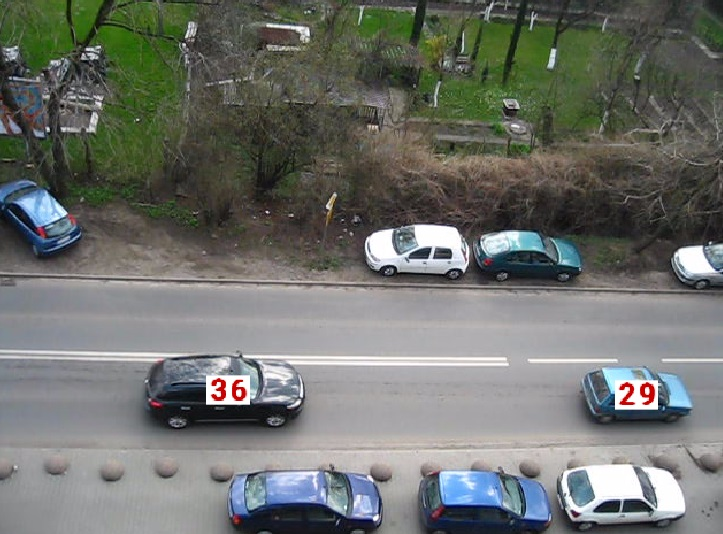
\includegraphics[width = \www \linewidth]{img6}%
	}%
	\hfill%
	\subfloat[\label{fig:montazSilniki}]{%
		\includegraphics[width = \www \linewidth]{img16}%
	}%
	
	\subfloat[\label{fig:montazKoloSwobodne}]{%
		\includegraphics[width = \www \linewidth]{img25}%
	}%
	\hfill%
	\subfloat[\label{fig:montazKola}]{%
		\includegraphics[width = \www \linewidth]{img30}%
	}%
	\hfill%
	\subfloat[\label{fig:montazBaterie}]{%
		\includegraphics[width = \www \linewidth]{img36_2}%
	}%
	
	\subfloat[\label{fig:montazKoszyk}]{%
		\includegraphics[width = \www \linewidth]{img39}%
	}%
	\hfill%
	\subfloat[\label{fig:montazArduino}]{%
		\includegraphics[width = \www \linewidth]{img42}%
	}%
	\hfill%
	\subfloat[\label{fig:montazShield}]{%
		\includegraphics[width = \www \linewidth]{img46}%
	}%
	
	\subfloat[\label{fig:montazSensory}]{%
		\includegraphics[width = \www \linewidth]{img58}%
	}%
	\hfill%
	\subfloat[\label{fig:montazSensory2}]{%
		\includegraphics[width = \www \linewidth]{img62}%
	}%
	\hfill%
	\subfloat[\label{fig:montazKable}]{%
		\includegraphics[width = \www \linewidth]{img60}%
	}%

	\caption{Montaż \label{fig:montaz}}
\end{figure}

Montaż został rozpoczęty od przykręcenia kilku śrubek z podkładkami zwykłymi, sprężystymi i tulejami dystansowymi do podwozia (rys. nr \ref{fig:montazPodwozie}, \ref{fig:montazPodwozie2}). W następnych krokach te połączenia zostały wykorzystane do montażu innych części.

Następnie, na przód platformy zamontowane zostały silniki. W tym celu zostały wykorzystane dłuższe śrubki (30 mm), nakrętki oraz 4 małe części ze sklejki (rys. nr \ref{fig:montazSilniki}).

Z tyłu platformy, na środku, zamontowane zostało swobodne koło, które jest ciągnięte przez pojazd (rys. nr \ref{fig:montazKoloSwobodne}). Większe koła z gumowymi oponami, które napędzane są przez silniki, zostały następnie nałożone na osie silników (rys. nr \ref{fig:montazKola}).

Do koszyka zostały włożonych 6 baterii AA, a następnie koszyk został umieszczony na środku platformy (rys. nr \ref{fig:montazBaterie}). Tak położony koszyk oczywiście nie ma prawa się utrzymywać, gdy pojazd się porusza, dlatego został on przykręcony przez element ze sklejki (rys. nr \ref{fig:montazKoszyk}).

Na przód podwozia, korzystając z 3 tulei dystansowych -- zamontowanych w pierwszym kroku -- przykręcona została płytka Arduino Uno (rys. nr \ref{fig:montazArduino}), a na nią nałożona została nakładka (rys. nr \ref{fig:montazShield}). Do nakładki podłączone zostały przewody zasilające silniki, oraz przewód pochodzący od koszyka z bateriami.

Na tym etapie, pojazd jest w stanie poruszać się w sposób nieautonomiczny, tzn. może wykonywać zaprogramowane ruchy. Oczywiście, w tym celu należy wpierw podłączyć Arduino z komputerem i wgrać odpowiedni kod.

Na samym końcu, zamontowane zostały czujniki. Sensory znajdują się na samym przodzie platformy, a przymocowanie ich za pomocą dłuższych (25 mm) tulei dystansowych powoduje, że są one umieszczone tuż nad ziemią, co pozwala im dobrze śledzić linię (rys. nr \ref{fig:montazSensory}). Czujniki analogowe i cyfrowe zostały rozmieszczone w trochę inny sposób (rys. nr \ref{fig:montazSensory2}), co wynika z faktu, że pełnią trochę inne zadania:
\begin{itemize}
\item czujniki analogowe znajdują się blisko siebie, zostały ustawione pod pewnym kątem, tak by były w stanie objąć (oba naraz) linię na podłodze,
\item czujniki cyfrowe znajdują się bardziej po bokach, na zewnętrznych stronach platformy, a dodatkowo są umieszczone dalej, bardziej do przodu niż sensory analogowe.
\end{itemize}

Ze względu na fakt, że pod spodem pojazdu znajduje się wiele przewodów zostały one objęte przez gumkę recepturkę (rys. nr \ref{fig:montazSensory2}). Połączenie przewodów z Arduino (a właściwie z~nakładką) widać na ostatnim zdjęciu \ref{fig:montazKable}.

Gotowy pojazd został przedstawiony na rysunku nr \ref{fig:pojazd} poniżej.

\begin{figure}[h!]
	\centering
	\includegraphics[width = 0.7 \linewidth]{imgPojazd}
	\caption{Gotowa konstrukcja robota \label{fig:pojazd}}
\end{figure}

\subsection{Okablowanie}

Następnie połączono odpowiednie elementy z odpowiednimi pinami znajdującymi się na shieldzie Arduino (rys. nr \ref{fig:okablowanie}). Połączenia są następujące:
\begin{itemize}
\item Gniazda związane z zasilaniem silników oraz koszykiem z bateriami (rys. nr \ref{fig:kableV}), do tych gniazd doprowadzane są po dwa przewody. W przypadku silników (gniazda po prawej), ich kolejność nie ma znaczenia -- na etapie pisania programu będzie można łatwo ,,naprawić'' połączenie przewodów na odwrót. W przypadku koszyka z bateriami (gniazdo po lewej) polaryzacja jest ważna. W przypadku przypadkowego niepoprawnego połączenia przed spaleniem elektroniki powinien uratować nas bezpiecznik.
\item Każdy z czujników analogowych (rys. nr \ref{fig:kableAnal}) ma 3 przewody: zasilania, masy i sygnału. Na shieldzie znajdują się specjalnie przygotowane do obsługi tych czujników miejsca (na górze i na dole). Poza tym, na płytce znajdują się inne piny do obsługi sygnałów analogowych.
\item Podobnie jak w przypadku czujników analogowych, sensory cyfrowe (rys. nr \ref{fig:kableDig}) także mają 3 takie same przewody. Różnica polega jednak na tym, że przewody ,,sygnałowe'' trafiają na piny cyfrowe, a nie analogowe. Sygnał cyfrowy jest bardziej ubogi od analogowego, bo daje tylko dwie możliwe wartości: logicznie prawdziwa lub fałszywa, ale ich obsługa przebiega znacznie szybciej, bo konwertowanie sygnału analogowego na liczby zabiera dużo czasu.
\end{itemize}

\begin{figure}[htbp!]
	\centering
	
	\subfloat[silniki, baterie \label{fig:kableV}]{%
		\includegraphics[width = \www \linewidth]{kable1}%
	}%
	\hfill%
	\subfloat[czujniki analogowe \label{fig:kableAnal}]{%
		\includegraphics[width = \www \linewidth]{kable2}%
	}%
	\hfill%
	\subfloat[czujniki cyfrowe \label{fig:kableDig}]{%
		\includegraphics[width = \www \linewidth]{kable3}%
	}%
	
	\caption{Połączenia \label{fig:okablowanie}}
\end{figure}

Przewody, które przenoszą informacje, zostają wykorzystane na etapie tworzenia aplikacji. Wykorzystane piny to:
\begin{itemize}
\item czujnik analogowy lewy: A1, czujnik analogowy prawy: A0,
\item czujnik cyfrowy lewy: 12, czujnik cyfrowy prawy: 8.
\end{itemize}

\subsection{Aplikacja}

W tym punkcie omówiony zostanie sposób działania systemu sterowania.
Podane zostaną listingi fragmentów kodu odpowiedzialnego za realizację sterowania. Kompletny kod został umieszczony na końcu raportu jako dodatek \ref{sec:kodEmb}. Kod ten jest bogaty w komentarze, ale w tym punkcie zostaną one usunięte jako że kluczowe części kodu zostaną osobno omówione, więc nie potrzeby dwukrotnie podawać tych samych informacji.

Algorytm odpowiadający za sterowanie pojazdem został pokazany na rysunku nr \ref{fig:algorytm}.

\begin{figure}[hbtp!]
	\centering
	\includegraphics[width = 0.7 \linewidth]{algorithm}
	\caption{Algorytm sterowania \label{fig:algorytm}}
\end{figure}

\begin{enumerate}
\item System sterowania rozpoczyna od odczytania informacji z czujników analogowych i cyfrowych. Te informacje zostają przypisane do odpowiednich zmiennych. Operacja wejścia/wyjścia są operacjami, które zajmują najwięcej czasu, dlatego w przypadku, w konkretnej iteracji algorytmu odczyt czujników musi występować tylko jeden raz. Jeśli kod kilkukrotnie korzysta z informacji sensorycznych, to odczytuje zmienne, a nie czyta na nowo wskazań czujników.

W przypadku czujników analogowych zapamiętywane są oba wskazania. W przypadku czujników cyfrowych zapamiętywana jest tylko informacja o tym, który sensor wskazał linię jako ostatni.
\begin{lstlisting}[firstnumber = 78]
leftSensor = analogRead(SENSOR_ANALOG_LEFT);
rightSensor = analogRead(SENSOR_ANALOG_RIGHT);

digSensor = digitalRead(SENSOR_DIGITAL_LEFT) ? SENSOR_DIGITAL_LEFT : digSensor;
digSensor = digitalRead(SENSOR_DIGITAL_RIGHT) ? SENSOR_DIGITAL_RIGHT : digSensor;
\end{lstlisting}

\item Ze wskazań czujników analogowych wyznaczana jest średnia arytmetyczna. Dzięki tej informacji system sterowania jest w stanie stwierdzić czy robot znajduje się na czarnej linii, czy na podłodze.
\begin{lstlisting}[firstnumber = 86]
meanSensor = (rightSensor + leftSensor) / 2.0;
\end{lstlisting}

\item Następnie średnia ta jest porównywana względem pewnej wartości progowej. Ta informacja jest bezpośrednio wykorzystywana do stwierdzenia czy robot ma podążać wzdłuż linii według reguły PD, czy powinien nawracać.
\begin{lstlisting}[firstnumber = 91]
if (meanSensor > TURN_MEAN) {
\end{lstlisting}
\end{enumerate}

\subsubsection*{Podążanie za linią}
Jeśli średnia jest wyższa od progu robot stara się podążać wzdłuż linii, wtedy:
\begin{enumerate}
\setcounter{enumi}{3}
\item Średnia arytmetyczna ze wskazań czujników analogowych wykorzystywana jest do wyznaczenia pewnej prędkości ,,bazowej'' \texttt{baseVel}. Na tym etapie, ta prędkość bazowa może być tylko pomniejszona. Za pomocą \texttt{\#define} w kodzie deklarujemy wartość stałą \texttt{BASE\_VEL}, która jest pożądaną prędkością bazową. Jeśli wskazania czujników analogowych są niższe od pewnej wartości progowej, prędkość bazowa jest liniowo zmniejszana. Chodzi o to, że jeśli robot wyjechał zbyt mocno -- ale cały czas będąc na niej -- poza linię, to jego pożądana prędkość jest zmniejszana, by zapobiec całkowitemu wyjechaniu poza nią, i by ,,upłynnić'' jego skręty.
\begin{lstlisting}[firstnumber = 94]
baseVel = meanSensor <= DOLNA_GRANICA ?
	map(meanSensor, PODLOGA_MEAN, DOLNA_GRANICA, PODLOGA_VEL, BASE_VEL) :
	BASE_VEL;
\end{lstlisting}

\item Ze wskazań czujników analogowych wyznaczany jest uchyb. Następnie uchyb ten jest liniowo przekształcany na zmiany prędkości. Dobrane zostały tutaj wartości 150 jako maksymalne możliwe różnice pomiędzy wskazaniami sensorów analogowych, które są przekształcane na maksymalne możliwe zmiany prędkości, czyli wyznaczoną wcześniej \texttt{baseVel}. Tak naprawdę, to przekształcenie mogłyby wykonywać nastawy regulatora PD, ale pozostaliśmy przy tym wariancie.
\begin{lstlisting}[firstnumber = 101]
error = map(rightSensor - leftSensor, -150, 150, -baseVel, baseVel);
\end{lstlisting}

\item Na podstawie uchybu wyznaczany jest sygnał sterujący \texttt{control}, który jest obliczany według reguły PD. Nastawy regulatora były dobierane metodą prób i błędów.
\begin{lstlisting}[firstnumber = 104]
control = P * error + D * (error - errorPrev);
\end{lstlisting}

Jeśli algorytm obliczył zbyt duży sygnał sterujący to jest on pomniejszany, tak by nie przekraczał wartości \texttt{baseVel}. Chodzi o to, by w najgorszym przypadku jedno z kół dostało prędkość równą 0, a nie ujemną.
\begin{lstlisting}[firstnumber = 108]
if (abs(control) > baseVel)
	control = control > 0 ? baseVel : -baseVel;
\end{lstlisting}

\item Sygnał sterujący modyfikuje pożądane prędkości kół. Kluczowy jest znak sygnału sterującego.
\begin{lstlisting}[firstnumber = 112]
leftVel = baseVel + control;
rightVel = baseVel - control;
\end{lstlisting}

\item Ostatecznie, tylko jedna prędkość ulega zmianie -- ta która została zmniejszona. Prędkość która wzrosła, jest sprowadzana na poziom \texttt{baseVel}.
\begin{lstlisting}[firstnumber = 117]
leftVel = leftVel > baseVel ? baseVel : leftVel;
rightVel = rightVel > baseVel ? baseVel : rightVel;
\end{lstlisting}
\end{enumerate}

\subsubsection*{Nawracanie}
Natomiast, jeśli średnia \texttt{meanSensor} była zbyt niska -- co oznacza, że robot lekko wyjechał poza linię -- system sterowania wyznacza prędkości, których celem jest nawrócenie, i powrót pojazdu na trasę.
\begin{enumerate}
\setcounter{enumi}{3}
\item Zmienna \texttt{digSensor} zapamiętuje, który sensor cyfrowy wykrył linię jako ostatni. Ta informacja jest wykorzystywana do wyznaczenia kierunku nawracania, a właściwie, wyznaczana jest pewna prędkość bazową nawracania \texttt{turnVel}%
\footnote{Ta zmienna jest nadmiarowa, równie dobrze w kodzie można było dla tego samego celu użyć zmiennej \texttt{baseVel}, która jest w tej gałęzi instrukcji \texttt{if} nieużywana.}%
, której znak jest zmieniany w zależności od wskazań sensorów cyfrowych.
\begin{lstlisting}[firstnumber = 122]
turnVel = digSensor == SENSOR_DIGITAL_LEFT ? -TURN_VEL : TURN_VEL;
\end{lstlisting}

\item Prędkość nawracania \texttt{turnVel} jest wykorzystywana do wyznaczenia faktycznych prędkości kół \texttt{leftVel}, \texttt{rightVel}. Prędkości muszą mieć różny znak, by ruch robota był realizowany w miejscu.

\item Dodatkowo prędkości te są przemnażane, by pojazd poruszał się nie tyle w miejscu, co wykonywał ruch do tyłu w odpowiednim kierunku. W ten sposób uwzględniany jest fakt, że w tym momencie robot jest poza linią.
\begin{lstlisting}[firstnumber = 127]
leftVel = turnVel < 0 ? turnVel * 1.5 : turnVel * 0.75;
rightVel = -turnVel < 0 ? -turnVel * 1.5 : -turnVel * 0.75;
\end{lstlisting}
\end{enumerate}

\subsubsection*{Dalsza część algorytmu}
Bez względu na to, która część algorytmu zadziałała, wyznaczone zostały pożądane prędkości kół \texttt{leftVel} i \texttt{rightVel}. Te prędkości są już podawane do osobnej funkcji \texttt{motor}, która zajmuje się generacją odpowiedniego sygnału PWM.
\begin{lstlisting}[firstnumber = 148]
void motor(int vel, byte leftRight) {
    byte dir = vel > 0 ? FORWARD : BACKWARDS;

    vel = map(abs(vel), 0, 100, 0, PWM_MAX);

    digitalWrite(leftRight == LEFT ? H_LEFT_DIR : H_RIGHT_DIR, dir);
    analogWrite(leftRight == LEFT ? H_LEFT_PWM : H_RIGHT_PWM, vel);
}
\end{lstlisting}

Funkcja jako argumenty przyjmuje: pożądaną prędkość w procentach (\texttt{vel}), oraz który silnik został wybrany (\texttt{leftRight}). Znak prędkości jest uwzględniany do wyboru kierunku (\texttt{dir}), a sama prędkość jest następnie liniowo przeskalowana na odpowiednie wypełnienie sygnału PWM (teraz już przetwarzana jest tylko jest wartość bezwzględna). Ostatnie dwie linijki związane są z obsługą mostku H:
\begin{itemize}
\item najpierw na odpowiedni pin mostka, podawany jest sygnał logicznie prawdziwy/fałszywy w zależności od pożądanego kierunku jazdy,
\item następnie na odpowiedni pin mostka, podawany jest sygnał PWM, który odpowiada za prędkość.
\end{itemize}

O co chodzi z \texttt{PWM\_MAX}? Nie chcemy by silniki były zasilane zbyt dużym napięciem, chcemy by maksymalnie było to 5V. Dla zdefiniowanej wartość \texttt{PWM\_MAX} sygnał o tym wypełnieniu dostarcza mniej więcej takie napięcie.

Jak widać, funkcja jest uniwersalna -- może obsługiwać oba silniki oraz prędkości w obie strony. Z tego powodu jest tu wiele różnych stałych związanych z mostkiem H, uwzględnieniem kierunku prędkości i uwzględnieniem wybranego silnika%
\footnote{Dokładne wartości wszystkich wspomnianych stałych są widoczne w listingu kodu.}.
Co najważniejsze, jest czytelna, i nie zajmuje wiele miejsca.\\

Na samym końcu zapamiętywany jest uchyb, by w następnej iteracji algorytmu został uwzględniony dla części D regulatora.
\begin{lstlisting}[firstnumber = 141]
errorPrev = error;
\end{lstlisting}

Cały omówiony algorytm realizowany jest cyklicznie w funkcji \texttt{loop}.

\subsection{Uwagi do aplikacji}

\subsubsection{Prędkości bazowe}
W kodzie znajdują się 3 zdefiniowane przez \texttt{\#define} prędkości bazowe:
\begin{itemize}
\item \texttt{BASE\_VEL} -- to pożądana prędkość ruchu w linii prostej,
\item \texttt{PODLOGA\_VEL} -- to pożądana prędkość ruchu w linii prostej, gdy robot nie znajduje się w całości na linii,
\item \texttt{TURN\_VEL} -- to prędkość bazowa dla nawracania.
\end{itemize}

\begin{lstlisting}[firstnumber = 49]
#define BASE_VEL 70
#define PODLOGA_VEL 20
#define TURN_VEL 40
\end{lstlisting}

Użycie prędkości \texttt{BASE\_VEL} i \texttt{PODLOGA\_VEL} znajdują się w tej samym miejscu w kodzie -- jest to fragment odpowiedzialny za ustalenie prędkości bazowej \texttt{baseVel}%
\footnote%
{Uwaga! \texttt{baseVel} to zmienna, której wartość ulega zmianie, a \texttt{BASE\_VEL} to wartość stała.}%
.
\begin{lstlisting}[firstnumber = 94]
baseVel = meanSensor <= DOLNA_GRANICA ?
	map(meanSensor, PODLOGA_MEAN, DOLNA_GRANICA, PODLOGA_VEL, BASE_VEL) :
	BASE_VEL;
\end{lstlisting}

Na rysunku nr \ref{fig:velocity} poniżej przedstawiony został kawałek wykresu przedstawiającego wpływ średniej z sensorów na prędkość bazową. Na wykresie zaznaczone zostały dwa punkty:
\begin{itemize}
\item (\texttt{DOLNA\_GRANICA}, \texttt{BASE\_VEL}) -- punkt określający dla jakiego wskazania, utrzymana jest stała prędkość \texttt{baseVel} równa \texttt{BASE\_VEL},
\item (\texttt{PODLOGA\_MEAN}, \texttt{PODLOGA\_VEL}) -- punkt określający nachylenie linii profilu prędkości.
\end{itemize}

\begin{figure}[h!]
	\centering
	\includegraphics[width = 0.4\linewidth]{velocity}
	\caption{Prędkość \texttt{baseVel} w funkcji średniej z sensorów \texttt{meanSensor} \label{fig:velocity}}
\end{figure}

\newpage

Natomiast prędkość \texttt{TURN\_VEL} wykorzystywana jest w przypadku dobierania prędkości nawracania \texttt{turnVel}.
\begin{lstlisting}[firstnumber = 122]
turnVel = digSensor == SENSOR_DIGITAL_LEFT ? -TURN_VEL : TURN_VEL;
\end{lstlisting}

Wszystkie 3 wspomniane prędkości stanowią pewne punkty odniesienia, które dostrajają robota do pracy w jego środowisku. Skąd konkretne wartości? Zostały dobrane metodą prób i błędów. Gdyby robot miałby przejechać trasę w innym miejscu, być może uległyby one pewnym zmianom.

\subsubsection{Charakterystyczne wskazania sensorów analogowych}
Podobnie jak w przypadku prędkości, zdefiniowane zostały 3 charakterystyczne wskazania czujników analogowych:
\begin{itemize}
\item \texttt{DOLNA\_GRANICA} -- dolne wskazanie czujnika analogowego, które cały czas oznacza przebywania ponad linią,
\item \texttt{TURN\_MEAN} -- średnia ze wskazań czujników, która przekroczona z dołu oznacza przebywanie poza linią i aktywny tryb nawracania,
\item \texttt{PODLOGA\_MEAN} -- średnia ze wskazań czujników charakterystyczna dla ,,podłogi'' (robot poza linią).
\end{itemize}

\begin{lstlisting}[firstnumber = 58]
#define DOLNA_GRANICA 620
#define TURN_MEAN 600
#define PODLOGA_MEAN 550
\end{lstlisting}

Pomiędzy tymi wartościami istnieje ścisła relacja:
\begin{equation*}
\texttt{PODLOGA\_MEAN} \quad < \quad \texttt{TURN\_MEAN} \quad < \quad \texttt{DOLNA\_GRANICA}
\end{equation*}

\begin{itemize}
\item Jeśli średnia jest ponad \texttt{DOLNA\_GRANICA} robot znajduje się na linii (dosyć centralnie ponad nią);
\item Jeśli średnia jest pomiędzy \texttt{DOLNA\_GRANICA}, a \texttt{TURN\_MEAN} robot znajduje się na linii, a zaczyna z niej wyjeżdżać, zatem zmniejszeniu ulega prędkość bazowa \texttt{baseVel};
\item Jeśli średnia jest poniżej \texttt{TURN\_MEAN} robot znajduje się poza linią, więc aktywowany zostaje tryb nawracania;
\item Punkt \texttt{PODLOGA\_MEAN} wykorzystywany jest przy liniowym zmniejszaniu prędkości (poprzedni punkt).
\end{itemize}

Te punkty dobierane są na etapie kalibracji robota (osobny punkt rozdziału).

\subsubsection{Nastawy regulatora}

Do wyznaczania sygnału sterującego wykorzystany został algorytm PD. Jego nastawy zostały dobrane metodą prób i błędów.
\begin{lstlisting}[firstnumber = 73]
float P = 0.9;
float D = 0.3;
\end{lstlisting}

Te wartości ulegały także zmianom, jeśli dobierane były inne prędkości bazowe. Dodatkowo warto wspomnieć o dwóch rzeczach:
\begin{enumerate}
\item Linijkę przed wyznaczaniem sygnału sterującego \texttt{control}, sygnał uchybu \texttt{error} jest liniowo przekształcany na pewien zakres prędkości. W klasycznym regulatorze, to nastawy odpowiadają za wszelkie przekształcanie uchybu, więc zastosowane nastawy uległy by pewnym zmianom. Nie miałoby to jednak większego znaczenia na działanie układu (zakładając, że zostaną dobrane odpowiednie nastawy).
\item W przypadku równania PD, człon D pomija wartość kroku czasowego, tzn. wzmocnienie D jest wymnażane przez różnicę pomiędzy uchybem aktualnym, a poprzednim, ale nie jest on dzielony przez krok czasowy $dt$. W zależności od ,,sytuacji'', kod może wykonywać się krócej lub dłużej, więc nie możemy tu wpisać pewnej stałej wartości czasu. Za pomocą pewnych funkcji można wyznaczyć ile wykonuje się fragment kodu, ale nie ma to większego znaczenia, bo może on ulegać zmianom. Krok czasowy został zatem uwzględniony we wzmocnieniu części D.
\end{enumerate}

\subsubsection{Sensory analogowe a cyfrowe}

Jak można zauważyć po punkcie analizującym kod systemu sterowania, sensory analogowe i cyfrowe są traktowane w inny sposób. Nie chodzi tutaj o samą oczywisty różnicę pomiędzy sygnałami, które zwracają Arduino, a o ich zadania w systemie sterowania:
\begin{itemize}
\item czujniki cyfrowe umieszczone są \emph{dalej} niż czujniki analogowe, ich zadaniem jest zapamiętywanie który czujnik wykrył linię jako ostatni i kluczowe jest to, że analizują przyszłe zdarzenia w stosunku do sensorów analogowych, które reagują na ,,teraźniejszość'',
\item informacja pochodząca z czujników analogowych jest wykorzystywana dużo częściej, można powiedzieć ,,cały czas'', bo na ich bazie wyznaczane są sygnały sterujące sprowadzające robota na trasę.
\end{itemize}

Czujniki cyfrowe są wykorzystywane tylko w przypadku gdy robot zjechał z linii, i należy wyznaczyć kierunek nawracania.

\subsection{Kalibracja}

Zanim robot będzie mógł realizować swoje zadania podążania wzdłuż linii musi zostać odpowiednio dostrojony do tego. Chodzi tutaj o:
\begin{itemize}
\item potencjometry czujników analogowych i cyfrowych,
\item dokładne wartości pewnych zdefiniowanych stał występujących w kodzie.
\end{itemize}

\subsubsection{Potencjometry}

Obsługa potencjometrów czujników cyfrowych jest dużo prostsza. Służą one do wyznaczenia pewnej wartości progowej odpowiedzialnej za różnicę pomiędzy zwracaniem wartości logicznie prawdziwej, a fałszywej. Prawdę mówiąc, po zainstalowaniu sensorów dokładne ustawienie tych potencjometrów nie ulegało zmianie. Różnice pomiędzy linią, a podłogą, są na tyle duże, że poza wstępnym ustawieniem tych potencjometrów, dalsze dostrajanie nie miało sensu.

Potencjometry czujników analogowych są dużo ważniejsze. Za ich pomocą możemy regulować jasność z jaką świeci dioda, coś zaś wpływa na inny zakres wartości liczbowych zwracanych do kodu Arduino. Ten zakres musi zostać odpowiednio dobrany do stałych występujących w kodzie (omówionych w poprzednich rozdziałach), ale dużo bardziej kluczowa jest inna sprawa -- oba czujniki muszą wskazywać mniej więcej to samo. Właśnie w kalibracji tych sensorów chodzi przede wszystkim o to, by oba czujniki wskazywały około te same wartości gdy znajdują się ponad podłogą albo ponad linią. Przyjmujemy tutaj pewien minimalny zakres dla różnic pomiędzy czujnikami, który nie wpływa znacząco na działanie układu%
\footnote{Dla małych różnic i tak wyznaczone sygnały sterujące zostaną następnie przez konwersję na liczby całkowitoliczbowe sprowadzone do zera.}, ale ważne jest żeby zwracać uwagę, że przy ,,tyrpnięciu'' robota ustawienie może ulec zmianie, przez co trzeba to naprawić.

Do kalibracji służy pewna funkcja w kodzie \texttt{sensorPrint}.
\begin{lstlisting}[firstnumber = 164]
void sensorPrint(void) {
    Serial.print("l: ");
    Serial.print(leftSensor);
    Serial.print(",  r: ");
    Serial.print(rightSensor);
    Serial.print(" ==> mean: ");
    Serial.println(meanSensor);
    delay(250);
}
\end{lstlisting}

Jej jedynym zadaniem jest wypisywanie na monitorze portu szeregowego wskazań sensorów analogowych oraz ich średniej co okres 250 ms. Należy przy tym także pamiętać o odkomentowaniu dwóch linijek w kodzie:
\begin{lstlisting}[firstnumber = 43]
//Serial.begin(9600);
\end{lstlisting}

\begin{lstlisting}[firstnumber = 138]
//sensorPrint();
\end{lstlisting}

Pierwsza z nich znajduje się w funkcji \texttt{setup}, która uruchamia się przy włączeniu Ardunio czy wgraniu nowego kodu i odpowiada za przygotowanie Arduino do przesyłu danych do monitora portu szeregowego. Druga linijka znajduje się w funkcji \texttt{loop} i jest to po prostu wywołanie wspomnianej wcześniej funkcji \texttt{sensorPrint}.

Przy kalibracji należy pamiętać o tym, by zworka zasilania silników była umieszczona w pozycji OFF (albo zupełnie ściągnięta), a Arduino pozostawało połączone poprzez kabel USB z komputerem. Następnie należy umieszczać pojazd w kilku różnych miejscach na podłodze i sprawdzać czy wskazania są podobne dla tych samych fragmentów podłoża. Jeśli tak nie jest, należy którymś z potencjometrów zmienić jasność diody. Na rysunku nr \ref{fig:kalibracja} widać ekran w trakcie kalibracji.

\begin{figure}[h!]
	\centering
	\includegraphics[width = 0.75 \linewidth]{kalibracja3_1}
	\caption{Monitor portu szeregowego \label{fig:kalibracja}}
\end{figure}

\subsubsection{Stałe występujące w kodzie}

Gdy poprzedni etap kalibracji jest zakończony przechodzimy do kolejnej części. Teraz chodzi o dobranie poprawnych wartości stałych: \texttt{PODLOGA\_MEAN}, \texttt{TURN\_MEAN} i \texttt{DOLNA\_GRANICA}, które poprawnie charakteryzują środowisku w którym będzie poruszał się robot. Cały czas korzystamy tutaj z poprzednio włączonego monitora portu szeregowego.

Stałe należy dobrać w następujący sposób:
\begin{enumerate}
\item Należy położyć robota w kilka różnych miejscach na podłodze, ale nie na linii. Podłogę będzie charakteryzował pewien zakres niższych wartości. Stała \texttt{PODLOGA\_MEAN} to po prostu około wartość w środku tego zakresu.
\item Stała \texttt{TURN\_MEAN} powinna być górną granicą zakresu charakteryzującego podłogę.
\item Należy położyć robota w kilku różnych miejscach ponad linią, by zbadać zakres wartości charakteryzujący sytuację gdy robot znajduje się ponad linią. Tym razem nie patrzymy na wartość średnią, a na wskazania obu sensorów. Jako stałą \texttt{DOLNA\_GRANICA} powinno dobrać się wartość dolnej granicy omawianego zakresu.
\end{enumerate}

\subsubsection{Stałe związane z prędkością i nastawy regulatora}
Należy także dobrać odpowiednie wartości stałych względem których dobierane są prędkości, czyli: \texttt{TURN\_VEL}, \texttt{BASE\_VEL} i \texttt{PODLOGA\_VEL} oraz nastawy regulatora PD, ale tutaj już nie ma ogólnych reguł. Jak zostało wspomniane w poprzednich punktach, wartości tych stałych były dobierane metodą prób i błędów. Ogólnie:
\begin{itemize}
\item zależy nam na tym, by line follower jak najszybciej pokonywał trasę, więc prędkości powinny być jak największe, ale ...
\item czym większe prędkości bazowe, tym trudniej jest układowi regulacji płynnie wyznaczać odpowiednie sygnały sprowadzające pojazd na trasę,
\item dodatkowo czym większe prędkości tym bardziej prawdopodobne, że robot opuści trasę, a wtedy już układ sterowania będzie starał się sprowadzać pojazd za pomocą trybu nawracania co znacznie spowalnia ruch.
\end{itemize}

\subsection{System FreeRTOS}
Ostatnim krokiem pracy była implementacja systemu sterowania przy pomocy systemu czasu rzeczywistego FreeRTOS.
Kompletny kod zaimplementowany na tym systemie został umieszczony, wraz z komentarzami, na końcu raportu jako dodatek \ref{sec:kodRtos}. Podobnie jak w poprzednich punktach, przy listingach fragmentów komentarze będą pomijane.

Schemat przepływu zaproponowanego rozwiązania został przedstawiony na rysunku nr \ref{fig:rtos}.

\begin{figure}[htbp!]
	\centering
	\includegraphics[width = 0.75\linewidth]{rtos_flowchart}
	\caption{Schemat przepływu \label{fig:rtos}}
\end{figure}

Kod, który poprzednio wykonywał się cyklicznie w funkcji \texttt{loop} został podzielony na 3 zadania:
\begin{itemize}
\item \texttt{taskSensors} -- zajmuje się odczytem wskazań czujników, pakuje je do struktury danych i wysyła poprzez kolejkę do \texttt{taskControl},
\item \texttt{taskControl} -- na podstawie danych sensorycznych wykonuje obliczenia odpowiedzialne za wyznaczenie pożądanych prędkości obu kół: \texttt{leftVel}, \texttt{rightVel}, a następnie umieszcza te prędkości w strukturze danych i przesyła za pomocą kolejki do \texttt{taskMotors},
\item \texttt{taskMotors} -- zadanie, które zajmuje się generacją odpowiednich sygnałów PWM wynikających z zadanych prędkości kół otrzymanych od poprzedniego zadania.
\end{itemize}

Zadania różnia się priorytetem: \texttt{taskSensors} ma najniższy (1), \texttt{taskControl} wyższy (2), a \texttt{taskMotors} najwyższy (3). Definicja zadań w systemie widoczna jest w listingu poniżej.
\begin{lstlisting}[firstnumber = 43]
xTaskCreate(
	taskSensors, "Obsluga czujnikow",
	128, NULL, 1, NULL
);
xTaskCreate(
	taskControl, "Regulacja",
	128, NULL, 2, NULL
);
xTaskCreate(
	taskMotors, "Obsluga silnikow",
	128, NULL, 3, NULL
);
\end{lstlisting}

Wszystkie 3 zadania otrzymują stos o rozmiarze 128 słów.

Jak zostało wspomniane, zadania komunikują się ze sobą poprzez kolejki. W tym celu zostały utworzone dwie kolejki:
\begin{itemize}
\item \texttt{sensorQueue} -- wymiana danych sensorycznych:
\begin{equation*}
\texttt{taskSensors} \ \text{(nadawca)} \quad \rightarrow \quad \texttt{taskControl} \ \text{(odbiorca)}
\end{equation*}

\item \texttt{controlQueue} -- wymiana danych sterowania:
\begin{equation*}
\texttt{taskControl} \ \text{(nadawca)} \quad \rightarrow \quad \texttt{taskMotors} \ \text{(odbiorca)}
\end{equation*}
\end{itemize}

Kolejki mogą pomieścić 10 wiadomości, a te są przesyłane poprzez konkretne struktury: \texttt{sensorStruct}, \texttt{controlStruct}. Ich nazwy jasno wskazują do jakich kolejek trafiają takie paczki danych.
\begin{lstlisting}[firstnumber = 24]
struct sensorStruct {
    int leftSensor, rightSensor;
    byte digSensor;
};

struct controlStruct {
    int leftVel, rightVel;
};
\end{lstlisting}

Definicja kolejek:
\begin{lstlisting}[firstnumber = 37]
sensorQueue = xQueueCreate(10, sizeof(struct sensorStruct));
controlQueue = xQueueCreate(10, sizeof(struct controlStruct));
\end{lstlisting}

Sam algorytm sterowania nie uległ zmianie -- zaproponowane rozwiązanie korzystające z systemu FreeRTOS jest ,,tłumaczeniem'' tego co zostało napisane dla systemu wbudowanego na wspomniany system czasu rzeczywistego.
Z tego powodu, nie został wykorzystany cały potencjał FreeRTOSa i robot po zastosowaniu takiego kodu nie działa lepiej, a po prostu tak samo. Trzeba mieć na uwadze 2 kwestie:
\begin{enumerate}
\item Zaproponowany system sterowania nie jest szczególnie skomplikowany są tylko 4 czujniki, 2 silniki i pewne obliczenia ,,pomiędzy''. Do wykorzystania takiego sprzętu spokojnie wystarcza system wbudowany. Co prawda, system czasu rzeczywistego pozwala dużo lepiej panować nad tym, kiedy działają które fragmenty kodu i prawdopodobnie można by usprawnić nawet zaproponowane rozwiązanie, które nie jest szczególnie skomplikowane, ale...
\item Na wykorzystanie systemu FreeRTOS wykorzystany zostało tylko ostatni tydzień prac nad projektem. Było to zbyt mało czasu, by dobrze zapoznać się z możliwościami systemu.
\end{enumerate}

\newpage

\section{Rezultat}

Ogólnie rzecz mówiąc, robot poprawnie radzi sobie z zadaniem, które miał wykonywać, czyli podążać za linią. Co więcej, skromnym zdaniem autorów robot jeździ znacznie płynniej i szybciej od ,,konkurencji'', które prezentowała swoje rozwiązania w trakcie ostatnich zajęć projektowych%
\footnote{Co więcej, w porównaniu do większości wspomnianej konkurencji, autorzy prezentowali wyniki na żywo, a nie w postaci nagrań, które równie dobrze mogły zostać przygotowane dla mniej pewnych i bezpiecznych nastaw, dających lepsze rezultate (ale z pewnym prawdopodobieństwem, że coś może się nie udać}%
.

Materiały wideo (te same co rozdziale ,,Harmonogram''), pokazujące finalne działanie robota umieszczone są w linkach poniżej:
\begin{itemize}
\item \href{https://youtu.be/4WTrk285v4s}{https://youtu.be/4WTrk285v4s}
\item \href{https://youtu.be/nwpjGGdDjxc}{https://youtu.be/nwpjGGdDjxc}
\end{itemize}

Trasa, którą line follower miał pokonywać była znana od początku zajęć projektowych. Jest ona widoczna na rysunku \ref{fig:trasa}.
\begin{figure}[htbp!]
	\centering
	
	\subfloat[]{%
		\includegraphics[width = 0.45 \linewidth]{trasa}%
	}%
	\hfill%
	\subfloat[]{%
		\includegraphics[width = 0.45 \linewidth]{trasa2}%
	}%
	
	\caption{Trasa \label{fig:trasa}}
\end{figure}

Można tu dostrzec kilku kluczowych punktów, z którym robot musiał sobie poradzić:
\begin{itemize}
\item przecięcie na środku trasy,
\item ostre skręte o 90 stopni,
\item długi skręt po łuku,
\item poza tym, musi także umieć pokonać ją w obu kierunkach.
\end{itemize}

Omawiany robot potrafi poradzić sobie ze wspomnianymi punktami:
\begin{itemize}
\item Przecięcie na środku trasy nie robi większego problemu. Co prawda, po przejechaniu tego punktu robot przez chwilę oscyluje wokół trasy, ale są one momentalnie tłumione i nie powodują większych problemów. Podczas testów nie zdarzyło się ani razu, by pojazd wjechał na nie właściwą część trasy na skrzyżowaniu.
\item Skręt po łuku także nie jest większym problemem, robot płynnie pokonuje tę część trasy.
\item Przez pewien (krótki) czas, problem stanowił skręt o 90 stopni. Na początku prac, zaproponowany został robot wyposażony w dwa czujniki analogowe na przodzie, które w zupełności wystarczają do pokonania całej trasy, poza tymi dwoma punktami ostrych skrętów. Po kupnie i instalacji dwóch czujników cyfrowych (i napisaniu odpowiedniego kodu), te fragmenty także przestały stanowić problem. Algorytm sterowania stara się podążać wzdłuż linii -- korzystając z czujników analogowych -- a gdy lekko za nią wyjeżdża, bo nie jest w stanie za pomocą tych dwóch czujników zrealizować płynne skrętu o taki kąt, czujniki cyfrowe informują o tym, który jako ostatni wykrył linię i robot zaczyna nawracać w odpowiednim kierunku. Następnie, gdy znajduje już się na trasie, aktywowany ponownie jest tryb sterowania według reguły PD.
\item Wykonanie trasy w obie strony nie stanowi żadnego problemu.
\end{itemize}

Trasa nie stanowi żadnego problemu dla omawianego pojazdu. Zakładamy tu oczywiście, że poprawnie został przeprowadzony etap kalibracji (poprzedni punkt rozdziału), gdyż w przypadku dobrania nieodpowiednich wartości dla stałych występujących w kodzie i nastaw regulatora, robot nie wykonuje już swojego zadania tak płynnie jak powinien.
\begin{itemize}
\item Przy większych pożądanych prędkościach (stałe prędkości bazowych) robotowi może zdarzyć się wyjechanie podczas trasy. Wtedy aktywowany jest tryb nawracania, który poza ostrymi skrętami w narożnikach nie powinien być aktywowany, bo znacznie zwiększa to czas pokonania trasy.
\item Przy niewłaściwych nastaw regulatora PD robot może albo w ogóle nie nadążać za zmianami na trasie (i ją opuszczać) albo może reagować zbyt gwałtownie. Jeśli za cel stawiamy sobie pokonać trasę jak najszybciej, to lepiej jest by reagował zbyt gwałtownie na zmiany trasy, ale robot wtedy porusza się dosyć nieelegancko -- wykonuje bardzo gwałtowne skręty.
\end{itemize}

\newpage

\section{Podsumowanie}

Podsumowując, projekt skończył się sukcesem -- robot dobrze wykonywał swoje zadanie. Można się jednak przyczepić do kilku fragmentów pracy:
\begin{itemize}
\item Wykorzystane w pracy silniki z kołami nie zawierają enkoderów. Powoduje to, że system nie zna prędkości z jakimi faktycznie kręcą się kołami, co ma wpływ na dokładność systemu. Założono jednak, że ta nieznajomość będzie traktowana jako pewne zakłócenie działające na obiekt podlegający regulacji, które jest skutecznie tłumione przez sygnały sterujące. Prawdopodobnie, robot stracił na tym pewną dokładność, ale i tak działał zadowalająco dobrze.
\item Przez większość czasu robot korzysta tylko z dwóch sensorów analogowych do wyznaczania odpowiednich poprawek prędkości. Można cieszyć się z tego, że tak mała ilość informacji starcza do wyznaczania poprawnych sterowań, ale z drugiej strony gdyby zastosować większą ilość sensorów, można by mocniej wpłynąć na poprawne sterowanie. Nawet dodanie choćby jednego sensora analogowego (np. na środek dziobu platformy, pomiędzy dwa pozostałe czujniki) mogłoby znacząco usprawnić układ regulacji. Z drugiej jednak strony dodanie kolejnych sensorów analogowych znacząco zwiększa czas wykonywania się kodu, więc to też należałoby mieć na uwadze...
\item Być może zatem, najlepiej byłoby skorzystać z większej ilości czujników cyfrowych, ale wtedy dużej zmianie musiałby ulec zaproponowany system sterowania.
\item Czujniki cyfrowe wykorzystywane są tylko i wyłącznie do wyznaczenia kierunku nawracania. Być może, umieszczenie ich w innym miejscu, pozwoliłoby na wykorzystywanie ich razem z czujnikami analogowymi do wyznaczania sygnałów sterujących w trakcie podążania za linią.
\end{itemize}

Wymienione wyżej uwagi należy jednak bardziej rozumieć jako ,,pomysły na przyszłość'', które zostałyby zrealizowane gdyby autorzy ponownie wykonywali swoją pracę.\\


Zajęcia projektowe stanowiły ważny punkt w semestrze. Projekty uczą najlepiej, bo pokazują na ile teorie omawiane w trakcie wykładów mogą zostać zastosowane do rozwiązań prawdziwych rzeczywistych problemów. Projekty pokazują także, że wspomniane teorie stanowią pewne uproszczone modele rzeczywistych zagadnień i nie zawsze sprawdzą się w całości w rzeczywistości. Jako przykład można choćby podać ruch pojazdu do przodu -- należy po prostu podać na oba koła (zakładając napęd różnicowy) tę samą prędkość, by robot poruszał się do przodu ze stałą prędkością. Łatwo można się przekonać, że cała konstrukcja mechaniczna ma duży wpływ na ten ruch, i ruch idealnie po linii prostej jest bardzo trudno uzyskać.

Projekt pokazuje także, że rozwiązań jednego problemu jest mnóstwo i wybrane zależy głównie od preferencji autorów: pojazd może mieć różną ilość kół, platforma może mieć inny kształt, czujniki mogą zostać zamontowane w różnych miejscach podwozia, jak i same czujniki mogą działać na różnych zasadach czy wreszcie sam kod może zostać napisany na wiele różnych sposobów korzystając z systemu wbudowanego lub systemu czasu rzeczywistego -- jest tu dużo miejsca na kreatywność.

\emph{Last but not least}, projekt był ważny, bo w czasach chińskiego wirusa, gdy cała nauka działa w trybie zdalnym, i większość zajęć to głównie siedzenie przed komputerem, każdy kontakt z rzeczywistym sprzętem zyskuje dwukrotnie na swojej wartości.

\newpage

\pagenumbering{gobble}

\phantom{a}


%%%
%%%		DODATKI
%%%

\newpage

\pagenumbering{roman}
\begin{appendices}
\section{Pełny kod -- system wbudowany \label{sec:kodEmb}}


\linespread{1.0}

\begin{lstlisting}[basicstyle = \ttfamily \footnotesize]
// Line follower -- system wbudowany
// Sekcja nr 1:
//    Maksymilian Skibiński,
//    Paweł Kaźmieruk.
// AiR S2-I/Rob, 2021 r.

// Obsługa mostku H.
#define H_LEFT_PWM 5
#define H_LEFT_DIR 4
#define H_RIGHT_PWM 6
#define H_RIGHT_DIR 9

// Oznaczenie kierunku ruchu na bazie znaku prędkości.
#define FORWARD 0
#define BACKWARDS 1

// Oznaczenie położenia silnika.
#define LEFT 0
#define RIGHT 1

// Maksymalne dozwolone wypełnienie sygnału PWM.
#define PWM_MAX 165

// Piny sensorów analogowych.
#define SENSOR_ANALOG_LEFT A1
#define SENSOR_ANALOG_RIGHT A0

// Piny sensorów cyfrowych.
#define SENSOR_DIGITAL_LEFT 12
#define SENSOR_DIGITAL_RIGHT 8

void setup() {
    // Deklaracja pinów mostka H.
    pinMode(H_LEFT_DIR, OUTPUT);
    pinMode(H_RIGHT_DIR, OUTPUT);
    pinMode(H_LEFT_PWM, OUTPUT);
    pinMode(H_RIGHT_PWM, OUTPUT);

    // W przypadku, gdy chcemy komunikacji robota z komputerem,
    // by odczytać sensory na ekranie, aktywujemy taką komunikację
    // linijką poniżej.
    
    //Serial.begin(9600);
}


// Prędkości względem których algorytm sterowania
// oblicza używane prędkości.
#define BASE_VEL 70
#define PODLOGA_VEL 20
#define TURN_VEL 40

// Kluczowe wskazania sensorów analogowych. Zależą one,
// głównie od warunków ,,podłogowych'':
//    - DOLNA_GRANICA to troche ponad dolna granica wskazania na lini,
//    - TURN_MEAN to troche ponad wskazanie podlogowe,
//    - PODLOGA_MEAN to srednia ze wskazan na podlodze.
#define DOLNA_GRANICA 620
#define TURN_MEAN 600
#define PODLOGA_MEAN 550

// Zmienne:
//    - digSensor -- zapamiętuje, który sensor cyfrowy wskazał jako ostatni,
//    - wskazania czujników analogowych i ich średnia,
//    - zmienne zapamiętujące wyznaczane prędkości,
//    - zmienne algorytmu sterowania.
byte digSensor = 0;
int leftSensor, rightSensor, meanSensor;
int baseVel, leftVel, rightVel, turnVel;
int control, error, errorPrev = 0;

// Nastawy regulatora PD.
float P = 0.9;
float D = 0.3;

void loop() {
    // Odczyt sensorów analogowych.
    leftSensor = analogRead(SENSOR_ANALOG_LEFT);
    rightSensor = analogRead(SENSOR_ANALOG_RIGHT);

    // Zmienna digSensor zapamiętuje, który sensor cyfrowy wykrył linię jako ostatni.
    digSensor = digitalRead(SENSOR_DIGITAL_LEFT) ? SENSOR_DIGITAL_LEFT : digSensor;
    digSensor = digitalRead(SENSOR_DIGITAL_RIGHT) ? SENSOR_DIGITAL_RIGHT : digSensor;

    // Średnia z pomiarów czujników analogowych.
    meanSensor = (rightSensor + leftSensor) / 2.0;
        
    // W zależności od wskazania średniego sensorów analogowych robot:
    //    - realizuje sterowanie według regulatora PD,
    //    - realizuje nawracanie.
    if (meanSensor > TURN_MEAN) {
        // ,,Prędkość bazowa'' -- jeśli średnia z sensorów jest za niska to pr. bazowa 
        // zostaje zmniejszona, bo oznacza to, że pojazd nie jest ponad linią.
        baseVel = meanSensor <= DOLNA_GRANICA ?
            map(meanSensor, PODLOGA_MEAN, DOLNA_GRANICA, PODLOGA_VEL, BASE_VEL)
            : BASE_VEL;
    
        // Uchyb z sensorów analogowych, który jest od razu liniowo przekształcany
        // na zmiany prędkości (równie dobrze nastawy regulatora
        // mogłyby się tym zająć).
        error = map(rightSensor - leftSensor, -150, 150, -baseVel, baseVel);
    
        // Sygnał sterujący regulatora PD.
        control = P * error + D * (error - errorPrev);
    
        // Ograniczenie górne -- jeśli sygnał sterujący jest
        // zbyt duży to stosujemy gorną granicę.
        if (abs(control) > baseVel)
            control = control > 0 ? baseVel : -baseVel;
    
        // Sygnał sterujący trafia na oba koła z innym znakiem.
        leftVel = baseVel + control;
        rightVel = baseVel - control;
    
        // Chcemy jedynie zmniejszyć jedną z prędkości, zatem jeśli, któraś
        // wzrosła to wraca ona na poziom prędkości ,,bazowej''.
        leftVel = leftVel > baseVel ? baseVel : leftVel;
        rightVel = rightVel > baseVel ? baseVel : rightVel;
    } else {
        // W zależności od tego, który sensor cyfrowy wykrył linię jako ostatni
        // wyznaczany jest odpowiedni kierunek zwrotu.
        turnVel = digSensor == SENSOR_DIGITAL_LEFT ? -TURN_VEL : TURN_VEL;

        // Robot nie wykonuje obrotu w miejscu, bo znajduje się trochę za linią
        // dlatego podawane prędkości są odpowiednio przemnażane, by
        // obrócił się oraz wrócił do tyłu.
        leftVel = turnVel < 0 ? turnVel * 1.5 : turnVel * 0.75;
        rightVel = -turnVel < 0 ? -turnVel * 1.5 : -turnVel * 0.75;        
    }

    // Ostatecznie, prędkości trafiają do silników.
    motor(leftVel, LEFT);
    motor(rightVel, RIGHT);    

    // Jeśli chcemy odczytać sensory na komputerze, to
    // wykorzystujemy zakomentowaną funkcję.
    
    //sensorPrint();

    // Uchyb poprzedni, dla następnej iteracji.
    errorPrev = error;
}

// Funkcja do przekazywania sygnału sterowania na silniki.
// Przyjmuje dwa argumenty:
//    - vel -- prędkość zadana w procentach, uwzględniany jest znak,
//    - leftRight -- który silnik.
void motor(int vel, byte leftRight) {
    // Uwzględnienie kierunku.
    byte dir = vel > 0 ? FORWARD : BACKWARDS;

    // Przekształcenie prędkości w procentach,
    // na użytkowany zakres sygnału PWM.
    vel = map(abs(vel), 0, 100, 0, PWM_MAX);

    // Ostatecznie, przypisanie prędkości wraz z obsługą mostka H.
    digitalWrite(leftRight == LEFT ? H_LEFT_DIR : H_RIGHT_DIR, dir);
    analogWrite(leftRight == LEFT ? H_LEFT_PWM : H_RIGHT_PWM, vel);
}

// Funkcja zajmująca się wypisywaniem poprzez monitor portu szeregowego
// wskazań sensora, i ich średniej.
// Funkcja jest istotna na etapie ,,strojenia'' potencjometrów czujników analogowych.
void sensorPrint(void) {
    Serial.print("l: ");
    Serial.print(leftSensor);
    Serial.print(",  r: ");
    Serial.print(rightSensor);
    Serial.print(" ==> mean: ");
    Serial.println(meanSensor);
    delay(250);
}
\end{lstlisting}

\newpage



\section{Pełny kod -- system FreeRTOS \label{sec:kodRtos}}

\begin{lstlisting}[basicstyle = \ttfamily \footnotesize]
// Line follower -- system FreeRTOS
// Sekcja nr 1:
//    Maksymilian Skibiński,
//    Paweł Kaźmieruk.
// AiR S2-I/Rob, 2021 r.

// Ładujemy FreeRTOSa oraz obsługę kolejek.
#include <Arduino_FreeRTOS.h>
#include <queue.h>

// W kodzie tworzymy 3 zadania:
//    - taskSensors -- obsługa sensorów,
//    - taskControl -- generowanie sterowania na podstawie danych z sensorów,
//    - taskMotors -- podawanie sygnałów sterujących na silniki.
void taskSensors(void *pvParameters);
void taskControl(void *pvParameters);
void taskMotors(void *pvParameters);

// Pomiędzy zadaniami są 2 kolejki.
QueueHandle_t sensorQueue;
QueueHandle_t controlQueue;

// Paczka danych wysyłana przez taskSensors do taskControl.
struct sensorStruct {
    int leftSensor, rightSensor;
    byte digSensor;
};

// Paczka danych wysyłana przez taskControl do taskMotors.
struct controlStruct {
    int leftVel, rightVel;
};

void setup() {
    // Tworzymy dwie kolejki do wymiany danych o odpowiednich rozmiarach (w bajtach)
    // i założyliśmy kolejki o długości 10 wiadomości.
    sensorQueue = xQueueCreate(10, sizeof(struct sensorStruct));
    controlQueue = xQueueCreate(10, sizeof(struct controlStruct));

    // Jeśli kolejki zostały utworzone, tworzymy zadania.
    // Zadania różnią się priorytetem, gdzie 3 to najwyższy.
    if (sensorQueue != NULL && controlQueue != NULL) {
        xTaskCreate(
            taskSensors, "Obsluga czujnikow",
            128, NULL, 1, NULL
        );
        xTaskCreate(
            taskControl, "Regulacja",
            128, NULL, 2, NULL
        );
        xTaskCreate(
            taskMotors, "Obsluga silnikow",
            128, NULL, 3, NULL
        );        
    }
}

// Funkcja ,,loop'' jest teraz oczywiście pusta.
void loop() { }

// Piny sensorów analogowych.
#define SENSOR_ANALOG_LEFT A1
#define SENSOR_ANALOG_RIGHT A0

// Piny sensorów cyfrowych.
#define SENSOR_DIGITAL_LEFT 12
#define SENSOR_DIGITAL_RIGHT 8

// Zadanie taskSensors zajmuje się odczytem wskazań sensorów
// oraz przekazaniem ich poprzez kolejkę do następnego zadania.
void taskSensors(void *pvParameters) {

    for (;;) {
        struct sensorStruct sensorData;

        // Odczyt sensorów analogowych.
        sensorData.leftSensor = analogRead(SENSOR_ANALOG_LEFT);
        sensorData.rightSensor = analogRead(SENSOR_ANALOG_RIGHT);

        // Zmienna digSensor zapamiętuje, który
        // sensor cyfrowy wykrył linię jako ostatni.
        sensorData.digSensor =
            digitalRead(SENSOR_DIGITAL_LEFT) ? SENSOR_DIGITAL_LEFT
            : sensorData.digSensor;
        sensorData.digSensor =
            digitalRead(SENSOR_DIGITAL_RIGHT) ? SENSOR_DIGITAL_RIGHT
            : sensorData.digSensor;

        // Dane zostają przekazane dalej.
        xQueueSend(sensorQueue, &sensorData, portMAX_DELAY);
    }
}

// Prędkości względem których algorytm sterowania
// oblicza używane prędkości.
#define BASE_VEL 70
#define PODLOGA_VEL 20
#define TURN_VEL 40

// Kluczowe wskazania sensorów analogowych. Zależą one,
// głównie od warunków ,,podłogowych'':
//    - DOLNA_GRANICA to troche ponad dolna granica wskazania na lini,
//    - TURN_MEAN to troche ponad wskazanie podlogowe,
//    - PODLOGA_MEAN to srednia ze wskazan na podlodze.
#define DOLNA_GRANICA 620
#define TURN_MEAN 600
#define PODLOGA_MEAN 550

// Zadanie taskControl zajmuje się wygenerowaniem odpowiednich sygnałów
// sterujących, czyli prędkości dla obu silników.
// Następnie, te prędkości zostają przekazane do zadania taskMotors.
void taskControl(void *pvParameters) {
    // Zmienne:
    //    - meanSensor -- średnia z dwóch sensorów analogowych,
    //    - baseVel, turnVel -- prędkość bazowa dla ruchu wzdłuż linii, i obrotu,
    //    - zmienne algorytmu sterowania.
    int meanSensor;
    int baseVel, turnVel;
    int control, error, error_prev;
    float P, D;
    struct sensorStruct sensorData;

    // Inicjalizacja uchyba poprzedniego oraz nastaw regulatora.
    error_prev = 0;
    P = 0.9;
    D = 0.3;

    for (;;) {
        // Jeśli zadania otrzymało paczkę danych od sensora to kod jest realizowany.
        // W przeciwnym razie zadanie czeka.
        if (xQueueReceive(sensorQueue, &sensorData, portMAX_DELAY) == pdPASS) {
            struct controlStruct controlData;

            // Średnia z pomiarów czujników analogowych.
            meanSensor = (sensorData.rightSensor + sensorData.leftSensor) / 2.0;

            // W zależności od wskazania średniego sensorów analogowych robot:
            //    - realizuje sterowanie według regulatora PD,
            //    - realizuje nawracanie.
            if (meanSensor > TURN_MEAN) {
                // ,,Prędkość bazowa'' -- jeśli średnia z sensorów jest za niska
                // to pr. bazowa zostaje zmniejszona, bo oznacza to,
                // że pojazd nie jest ponad linią.
                baseVel = meanSensor <= DOLNA_GRANICA ?
                    map(meanSensor, PODLOGA_MEAN, DOLNA_GRANICA, PODLOGA_VEL, BASE_VEL)
                    : BASE_VEL;

                // Uchyb z sensorów analogowych, który jest od razu
                // liniowo przekształcany na zmiany prędkości
                // (równie dobrze nastawy regulatora mogłyby się tym zająć).
                error = map(sensorData.rightSensor - sensorData.leftSensor,
                	-150, 150, -baseVel, baseVel);

                // Sygnał sterujący regulatora PD.
                control = P * error + D * (error - error_prev);

                // Ograniczenie górne -- jeśli sygnał sterujący
                // jest zbyt duży to stosujemy gorną granicę.
                if (abs(control) > baseVel)
                    control = control > 0 ? baseVel : -baseVel;

                // Sygnał sterujący trafia na oba koła z innym znakiem.
                controlData.leftVel = baseVel + control;
                controlData.rightVel = baseVel - control;

                // Chcemy jedynie zmniejszyć jedną z prędkości, zatem jeśli, któraś
                // wzrosła to wraca ona na poziom prędkości ,,bazowej''.    
                controlData.leftVel =
                	controlData.leftVel > baseVel ?
                	baseVel : controlData.leftVel;
                controlData.rightVel =
                	controlData.rightVel > baseVel ?
                	baseVel : controlData.rightVel;
            } else {
                // W zależności od tego, który sensor cyfrowy wykrył linię jako ostatni
                // wyznaczany jest odpowiedni kierunek zwrotu.                
                turnVel =
                	sensorData.digSensor == SENSOR_DIGITAL_LEFT ?
                	-TURN_VEL : TURN_VEL;

                // Robot nie wykonuje obrotu w miejscu, bo znajduje się trochę za linią
                // dlatego podawane prędkości są odpowiednio przemnażane, by
                // obrócił się oraz wrócił do tyłu.
                controlData.leftVel = turnVel < 0 ? turnVel * 1.5 : turnVel * 0.75;
                controlData.rightVel = -turnVel < 0 ? -turnVel * 1.5 : -turnVel * 0.75;
            }

            // Dane zostają przekazane do następnego zadania.
            xQueueSend(controlQueue, &controlData, portMAX_DELAY);
            
            // Uchyb poprzedni, dla następnej iteracji.
            error = error_prev;
        }
    }
}


// Obsługa mostku H.
#define H_LEFT_PWM 5
#define H_LEFT_DIR 4
#define H_RIGHT_PWM 6
#define H_RIGHT_DIR 9

// Maksymalne dozwolone wypełnienie sygnału PWM.
#define PWM_MAX 165

// Oznaczenie kierunku ruchu na bazie znaku prędkości.
#define FORWARD 0
#define BACKWARDS 1

void taskMotors(void *pvParameters) {
    // Deklaracja pinów mostka H.
    pinMode(H_LEFT_DIR, OUTPUT);
    pinMode(H_RIGHT_DIR, OUTPUT);
    pinMode(H_LEFT_PWM, OUTPUT);
    pinMode(H_RIGHT_PWM, OUTPUT);

    struct controlStruct controlData;
    byte dir;

    for (;;) {
        // Jeśli zadanie otrzymało paczkę danych od taskControl, to kod
        // jest realizowany. W przeciwnym wypadku zadanie oczekuje.
        if (xQueueReceive(controlQueue, &controlData, portMAX_DELAY) == pdPASS) {
            // Najpierw silnik lewy.
            // Uwzględnienie kierunku.
            dir = controlData.leftVel > 0 ? FORWARD : BACKWARDS;

            // Przekształcenie prędkości w procentach,
            // na użytkowany zakres sygnału PWM.            
            controlData.leftVel = map(abs(controlData.leftVel), 0, 100, 0, PWM_MAX);
            digitalWrite(H_LEFT_DIR, dir);
            analogWrite(H_LEFT_PWM, controlData.leftVel);

            // Teraz to samo dla silnika prawego.
            dir = controlData.rightVel > 0 ? FORWARD : BACKWARDS;
            
            controlData.rightVel = map(abs(controlData.rightVel), 0, 100, 0, PWM_MAX);
            digitalWrite(H_RIGHT_DIR, dir);
            analogWrite(H_RIGHT_PWM, controlData.rightVel);
        }
    }    
}
\end{lstlisting}
\end{appendices}

\end{document}